\documentclass[english,notitlepage]{revtex4-1}  % defines the basic parameters of the document
%For preview: skriv i terminal: latexmk -pdf -pvc filnavn



% if you want a single-column, remove reprint

% allows special characters (including æøå)
\usepackage[utf8]{inputenc}
%\usepackage[english]{babel}

%% note that you may need to download some of these packages manually, it depends on your setup.
%% I recommend downloading TeXMaker, because it includes a large library of the most common packages.

\usepackage{physics,amssymb}  % mathematical symbols (physics imports amsmath)
\usepackage{graphicx}         % include graphics such as plots
\usepackage{xcolor}           % set colors
\usepackage{hyperref}         % automagic cross-referencing (this is GODLIKE)
\usepackage{tikz}             % draw figures manually
\usepackage{listings}         % display code
\usepackage{subfigure}        % imports a lot of cool and useful figure commands
\usepackage{float}
\usepackage{algorithm}
\usepackage[noend]{algpseudocode}
% defines the color of hyperref objects
% Blending two colors:  blue!80!black  =  80% blue and 20% black
\hypersetup{ % this is just my personal choice, feel free to change things
    colorlinks,
    linkcolor={red!50!black},
    citecolor={blue!50!black},
    urlcolor={blue!80!black}}

%% Defines the style of the programming listing
%% This is actually my personal template, go ahead and change stuff if you want
\lstset{ %
	inputpath=,
	backgroundcolor=\color{white!88!black},
	basicstyle={\ttfamily\scriptsize},
	commentstyle=\color{magenta},
	language=Python,
	morekeywords={True,False},
	tabsize=4,
	stringstyle=\color{green!55!black},
	frame=single,
	keywordstyle=\color{blue},
	showstringspaces=false,
	columns=fullflexible,
	keepspaces=true}


%% USEFUL LINKS:
%%
%%   UiO LaTeX guides:        https://www.mn.uio.no/ifi/tjenester/it/hjelp/latex/
%%   mathematics:             https://en.wikibooks.org/wiki/LaTeX/Mathematics

%%   PHYSICS !                https://mirror.hmc.edu/ctan/macros/latex/contrib/physics/physics.pdf

%%   the basics of Tikz:       https://en.wikibooks.org/wiki/LaTeX/PGF/TikZ
%%   all the colors!:          https://en.wikibooks.org/wiki/LaTeX/Colors
%%   how to draw tables:       https://en.wikibooks.org/wiki/LaTeX/Tables
%%   code listing styles:      https://en.wikibooks.org/wiki/LaTeX/Source_Code_Listings
%%   \includegraphics          https://en.wikibooks.org/wiki/LaTeX/Importing_Graphics
%%   learn more about figures  https://en.wikibooks.org/wiki/LaTeX/Floats,_Figures_and_Captions
%%   automagic bibliography:   https://en.wikibooks.org/wiki/LaTeX/Bibliography_Management  (this one is kinda difficult the first time)
%%   REVTeX Guide:             http://www.physics.csbsju.edu/370/papers/Journal_Style_Manuals/auguide4-1.pdf
%%
%%   (this document is of class "revtex4-1", the REVTeX Guide explains how the class works)


%% CREATING THE .pdf FILE USING LINUX IN THE TERMINAL
%%
%% [terminal]$ pdflatex template.tex
%%
%% Run the command twice, always.
%% If you want to use \footnote, you need to run these commands (IN THIS SPECIFIC ORDER)
%%
%% [terminal]$ pdflatex template.tex
%% [terminal]$ bibtex template
%% [terminal]$ pdflatex template.tex
%% [terminal]$ pdflatex template.tex
%%
%% Don't ask me why, I don't know.

\begin{document}
\title{Project 1 - FYS3150}      % self-explanatory
\author{René Ask and Benedicte Nyheim}          % self-explanatory
\date{\today}                             % self-explanatory
\noaffiliation                            % ignore this
                                          % marks the end of the abstracthttps://github.com/reneaas/fys2160.git
\maketitle                                % creates the title, author, date & abstract

\section{Introduction}
Differential equations show up in all branches of physics. While there exists a subset of such equations that permit closed-form solutions, the differential equations that emerge from the vast majority of real world problems require us to resort to approximation schemes simply because no such solution exists. This lack of existence prompts us to develop and estimate the error of numerical methods in order to study and assert the validity of our results. 

In this article we shall study, compare and contrast three methods of solving Poisson's equation by converting the problem into a linear tridiagonal matrix equation. The first algorithm we'll look at is a general one developed to solve a tridiagonal matrix equation where we do not assume much about the matrix elements aside from requiring that the matrix is indeed invertible. We will further specialize the algorithm for our particular matrix and benchmark the two methods for comparative purposes. We will also compare these two methods towards a more intricate method using LU-decomposition in combination with the normal forward- and backward-substitutions required by the special form of Gaussian elimination we'll need. We'll then compare these methods against solvers from the well-known package armadillo.
\section{Method}
The general form of the differential equation (DE) with Dirichlet boundary conditions we wish to solve is 
\begin{equation}\label{diff_eq}
	-u''(x) = f(x), \quad x \in (0,1), \quad u(0)=u(1)=0.
\end{equation}
To this end, we'll derive an approximation to the second derivative of a general continuous function $f(x)$ before we estimate the total error of the approximation. For simplicity, we'll assume that this function is analytic, that is, it has derivatives of all orders.
\subsection{Derivation of the approximation scheme and an upper-bound on its total error}

We start by Taylor expanding about some point $x$ 
\begin{equation}
	f(x+h) = f(x) + hf'(x) + \frac{h^2}{2!}f''(x) + \frac{h^3}{3!}f'''(x) + \frac{h^4}{4!}f^{(4)}(\xi_1),
\end{equation}
and 
\begin{equation}
	f(x-h) = f(x) - hf'(x) + \frac{h^2}{2!}f''(x) - \frac{h^3}{3!}f'''(x) + \frac{h^4}{4!}f^{(4)}(\xi_2),
\end{equation}
where $\xi_1 \in (x,x+h)$ and $\xi_2 \in (x-h,x)$. Adding the two equations and rearranging a bit we get 
\begin{equation}
	f''(x) = \frac{f(x+h)-2f(x) + f(x-h)}{h^2} - \frac{h^2}{4!}\left[f(\xi_1)-f(\xi_2)\right].
\end{equation}
To find the signed truncation error, we rewrite the equation as 
\begin{equation}
	f''(x) - \frac{f(x+h)-2f(x) + f(x-h)}{h^2} = -\frac{h^2}{24}\left[f^{(4)}(\xi_1)-f^{(4)}(\xi_2)\right].
\end{equation}
Before we proceed with the error analysis, we might as well pick $\xi \in (x-h,x+h)$ such that $f(\xi) = \max \{f(\xi_1),f(\xi_2)\}$ and multiply it by a factor $2$ at the right-hand side (RHS), that is
\begin{equation}
	f''(x) - \frac{f(x+h)-2f(x) + f(x-h)}{h^2} = -\frac{h^2}{12}f(\xi).
\end{equation}
Due to the fact that computers are unable to represent numbers exactly, the computed values can be written as $\bar{f}(x+h) = f(x+h)(1+\epsilon_1)$, $\bar{f}(x) = f(x)(1+\epsilon_2)$ and $\bar{f}(x-h) = f(x-h)(1+\epsilon_3)$. An upper-bound estimate of the global total error, that is, the truncation error and the error due to loss of precision is 
\begin{equation}
	\begin{split}
	\epsilon & = \abs{f'(x) - \bar{f}'(x)} \\
			 & = \abs{f''(x) - \frac{\bar{f}(x+h)-2\bar{f}(x) + \bar{f}(x-h)}{h^2}}\\
			 & = \abs{f''(x) - \frac{f(x+h)(1+\epsilon_1)-2f(x)(1+\epsilon_2) + f(x-h)(1+\epsilon_3)}{h^2}} \\
			 & = \abs{f''(x) - \frac{f(x+h)-2f(x) + f(x-h)}{h^2} - \frac{f(x+h)\epsilon_1 - 2f(x)\epsilon_2 + f(x-h)\epsilon_3}{h^2}} \\
			 & \leq \abs{-\frac{h^2}{12}f(\xi)- \frac{\epsilon_1 - 2\epsilon_2 + \epsilon_3}{h^2}\max_{\zeta \in (x-h,x+h)}f(\zeta)} \\
			 & \leq 
			 \frac{h^2}{12}\max_{\xi \in (x-h,x+h)}\abs{f^{(4)}(\xi)} + \frac{\abs{\epsilon_1} + 2\abs{\epsilon_2} + \epsilon_3}{h^2}\max_{\zeta \in (x-h,x+h)}\abs{f(\zeta)} \\
			 & \leq \frac{h^2}{12}\max_{\xi \in (0,1)}\abs{f^{(4)}(\xi)} + \frac{4\epsilon_M}{h^2}\max_{\zeta \in (0,1)}\abs{f(\zeta)}.
	\end{split}\frac{5}{2}V_0(P_0 - P_1)
\end{equation}
Furthermore, we set $\epsilon_M = \max\{\abs{\epsilon_1}, \abs{\epsilon_2}, \abs{\epsilon_3}\}$. Now let $M_1 \equiv \max_{\xi \in (0,1)}\abs{f^{(4)}(\xi)}$ and 
$m_2 \equiv \max_{\zeta \in (0,1)}\abs{f(\zeta)}$. Then the upper-bound estimate of the total error can neatly be written as
\begin{equation}
	\epsilon \leq \frac{h^2}{12}M_1 + \frac{4\epsilon_M}{h^2}M_2.
\end{equation}
Solving $\dv*{\epsilon}{h} = 0$ with respect to $h$ yields the optimal choice of step-size $h^*$ given as  
\begin{equation}\label{optimal_stepsize}
	h^* = \left(\frac{48\epsilon_M M_2}{M_1}\right)^{1/4}.
\end{equation}
We need to determine $M_1$ and $M_2$ to estimate $h^*$ for our particular closed-form solution to the differential equation. This function is 

\begin{equation}
	f(x) = 1-(1-e^{-10})x - e^{-10x},
\end{equation}
and solving $\dv*{f}{x} = 0$ yields 
\begin{equation}
	\zeta = -\frac{\ln(1-e^{-10}) - \ln(10)}{10},
\end{equation}
such that $M_2 = \abs{f(\zeta)}$.
Furthermore, $f^{(4)}(x) = -10^4\exp(-10x)$, hence we see that $M_1 \leq \lim\limits_{\xi \to 0}\abs{f^{(4)}(\xi)}$. For simplicity, we might as well just set $M_1 = \abs{f^{(4)}(0)}$. Then we obtain 
\begin{equation}
	h^* \approx \left(\frac{48\epsilon_M \abs{f(\zeta)}}{\abs{f^{(4)}(0)}}\right)^{1/4} \approx 4\times 10^{-5},
\end{equation}
where we set $\epsilon_M = 10^{-15}$. For our purposes, it's more convenient to express it in terms of the logarithm
\begin{equation}
	\log_{10}(h^*) \approx -4.4.
\end{equation}


\subsection{Approximate solution of the differential equation by the Thomas algorithm}
From the arguments above it's obvious that we can approximate the second derivative of a function $f(x)$ by 
\begin{equation}
	f''(x_i) \approx \frac{f(x_i+h) - 2f(x_i) + f(x_i-h)}{h^2} \equiv \frac{f_{i+1} - f_i + f_{i-1}}{h^2},
\end{equation}

Now, for our particular DE, we want to approximate the true solution $u(x)$ by the a function $v(x)$. Using the discretization from above, we can thus rewrite our DE as 
\begin{equation}
	-\frac{-v_{i+1}+v_{i-1} - 2v_i}{h^2} = f_i, \quad i=1,2,...,n,
\end{equation}
which may be rearranged into 
\begin{equation}\label{approx_1}
	2v_i - v_{i+1} - v_{i-1} = f_ih^2 \equiv q_i.
\end{equation}
From \eqref{approx_1} we can rewrite this into a matrix equation as follows 
\begin{equation}
	\begin{pmatrix}
	2v_1 - v_2 \\ 
	-v_1 + 2v_2 - v_3 \\ 
	\vdots \\
	2v_n - v_{n-1}
	\end{pmatrix}
	=
	\begin{pmatrix}
	2 & -1 & 0  & \cdots & 0 \\
	-1 & 2 & -1 & \cdots & 0 \\
	\vdots \\
	0 & \cdots & 0 & -1 & 2 
	\end{pmatrix}
	\begin{pmatrix}
	v_1 \\ v_2 \\ \vdots \\ v_n
	\end{pmatrix}
	= \begin{pmatrix}
	q_1 \\ q_2 \\ \vdots \\ q_n
	\end{pmatrix}.
\end{equation}
To solve the matrix equation we'll first develop a general algorithm based on forward- and backward substitution to solve the equation $A\vb*{x} = \vb*{q}$. 
Performing one step of Gaussian elimination on the following matrix yields 
\begin{equation}
	A =
	\begin{pmatrix}
	b_1 & c_1 & 0 & \cdots & \cdots & \cdots \\
	a_1 & b_2 & c_2 & 0  &\cdots & \cdots  \\ 
	0 & a_2 & b_3 & 0 & \cdots & \cdots \\
	\vdots & \vdots & \vdots & \vdots & \ddots & \vdots \\
	0 & 0 & \cdots & a_{n-2} & b_{n-1} & c_{n-1} \\
	0 & 0 & \cdots  & 0 & a_{n-1} & b_n
	\end{pmatrix}
	\sim 
	\begin{pmatrix}
	b_1 & c_1 & 0 & \cdots & \cdots & \cdots \\
	0 & b_2 - \frac{a_1}{b_1}c_1 & c_2 & 0  &\cdots & \cdots  \\ 
	0 & a_2 & b_3 & 0 & \cdots & \cdots \\
	\vdots & \vdots & \vdots & \vdots & \ddots & \vdots \\
	0 & 0 & \cdots & a_{n-2} & b_{n-1} & c_{n-1} \\
	0 & 0 & \cdots  & 0 & a_{n-1} & b_n
	\end{pmatrix}.
\end{equation}
Defining $\tilde{b_2} \equiv b_2 - (a_1/b_1)c_1$, we can perform another step
\begin{equation}
	\begin{pmatrix}
	b_1 & c_1 & 0 & \cdots & \cdots & \cdots \\
	0 & \tilde{b_2} & c_2 & 0  &\cdots & \cdots  \\ 
	0 & a_2 & b_3 & 0 & \cdots & \cdots \\
	\vdots & \vdots & \vdots & \vdots & \ddots & \vdots \\
	0 & 0 & \cdots & a_{n-2} & b_{n-1} & c_{n-1} \\
	0 & 0 & \cdots  & 0 & a_{n-1} & b_n
	\end{pmatrix}
	\sim
	\begin{pmatrix}
	b_1 & c_1 & 0 & \cdots & \cdots & \cdots \\
	0 & \tilde{b_2} & c_2 & 0  &\cdots & \cdots  \\ 
	0 & 0 & b_3 - \frac{a_2}{\tilde{b_2}}c_2 & 0 & \cdots & \cdots \\
	\vdots & \vdots & \vdots & \vdots & \ddots & \vdots \\
	0 & 0 & \cdots & a_{n-2} & b_{n-1} & c_{n-1} \\
	0 & 0 & \cdots  & 0 & a_{n-1} & b_n
	\end{pmatrix},
\end{equation}
and at this point it's pretty obvious that the general pattern for the forward-substitution is  
\begin{gather}
	b_i = b_i - \frac{a_{i-1}}{b_{i-1}}c_{i-1}, \qquad \text{for} \qquad i=2,3,...,n,\\
	q_i = y_i - \frac{a_{i-1}}{b_{i-1}}y_{i-1}, \qquad \text{for} \qquad i=2,3,...,n,
\end{gather}
where the second equation is simply performing the exact same operation on the RHS of the equation. 

Once this process in completed, we need to perform back-substitution to find $\vb*{x}$. At this point our equation will look as follows: 
\begin{equation}
		\begin{pmatrix}
	b_1 & c_1 & 0 & \cdots & \cdots & \cdots \\
	0 & \tilde{b}_2 & c_2 & 0  &\cdots & \cdots  \\ 
	0 & 0 & \tilde{b}_3 & 0 & \cdots & \cdots \\
	\vdots & \vdots & \vdots & \ddots & \vdots & \vdots \\
	0 & 0 & \cdots & 0 & \tilde{b}_{n-1} & c_{n-1} \\
	0 & 0 & \cdots  & 0 & 0 & \tilde{b}_n
	\end{pmatrix}
	\begin{pmatrix}
	x_1 \\ x_2 \\ x_3 \\ \vdots \\ x_{n-1} \\ x_n
	\end{pmatrix}
	=
	\begin{pmatrix}
	b_1x_1 + c_1x_2\\
	\tilde{b}_2x_2 + c_2x_3 \\
	\tilde{b}_3x_3 + c_3x_4 \\
	\vdots \\
	\tilde{b}_{n-1}x_{n-1} + c_{n-1}x_{n} \\
	\tilde{b}_nx_n
	\end{pmatrix}
	=
	\begin{pmatrix}
	\tilde{q}_1 \\ \tilde{q}_2 \\ \tilde{q}_3 \\ \vdots \\ \tilde{q}_{n-1} \\ \tilde{q}_n
	\end{pmatrix},
\end{equation}
so the general algorithm for the back-substitution is 


\begin{gather}
	x_i = \frac{q_i}{b_i}, \qquad \text{for} \qquad i = n,\\
	x_i = \frac{q_i - c_ix_{i+1}}{b_i},\qquad \text{for} \qquad i = n-1, n-2, ...,1.
\end{gather}




For our particular matrix, we know that $b_i = 2$ and $c_i = a_i = -1$, so we can specialize the algorithm. To see this, we first motivate the formula by 
\begin{gather}
	b_1 = b = 2, \\
	b_2 = b - 1/b_1 = 2 - \frac{1}{2} = \frac{3}{2},\\
	b_3 = b - 1/b_2 = 2 -\frac{1}{3/2} = 2 - \frac{2}{3} = \frac{4}{3},\\
	\vdots \\
	b_i = \frac{i+1}{i}, \qquad \text{for} \qquad i = 1,2,...,n, \\
	q_i = q_i + \frac{i-1}{i}q_{i-1}, \qquad \text{for} \qquad i = 1,2,...,n.
\end{gather}
For the solution $\vb*{x}$ we get the recursive relations
\begin{gather}
	x_n = \frac{n}{n+1}q_n, \\
	x_i = \frac{i}{i+1}(q_i + x_{i+1}), \qquad \text{for} \qquad i = n-1,n-2,...,1.
\end{gather}

\subsection{LU-decomposition, Forward- and Back-substitution}
To this end we will develop an algorithm based on the LU-decomposition $A = LU$:
\begin{equation} A= 
	\begin{pmatrix}
	b_1 & c_1 & 0 & \cdots & \cdots & \cdots \\
	a_1 & b_2 & c_2 & 0  &\cdots & \cdots  \\ 
	0 & a_2 & b_3 & 0 & \cdots & \cdots \\
	\vdots & \vdots & \vdots & \vdots & \ddots & \vdots \\
	0 & 0 & \cdots & a_{n-2} & b_{n-1} & c_{n-1} \\
	0 & 0 & \cdots  & 0 & a_{n-1} & b_n
	\end{pmatrix}
	= 
	\begin{pmatrix}
	1 & 0 & \cdots &  \cdots & \cdots & 0 \\
	\ell_2 & 1 & \cdots & \cdots & \cdots & 0 \\
	0 & \ell_3 & 1 & \cdots & \cdots & 0 \\
	\vdots & \vdots & \vdots & \ddots & \vdots \\
	0 & 0 & \cdots & \ell_{n-1} & 1 & 0 \\
	0 & 0 & \cdots &\cdots & \ell_n & 1  
	\end{pmatrix}
	\begin{pmatrix}
	d_1 & u_1 & \cdots & \cdots &\cdots & 0 \\ 
	0 & d_2 & u_2 & \cdots & \cdots & 0 \\
	0 & 0 & d_3 & u_3 & \cdots & 0 \\
	\vdots & \vdots & \vdots & \ddots & \vdots & \vdots \\
	0 & 0 & \cdots & \cdots & d_{n-1} & u_{n-1} \\
	0 & 0 & \cdots & \cdots & 0 & d_n
	\end{pmatrix}
	= LU,
\end{equation}
and performing matrix multiplication we get 
\begin{equation}
	LU = 
	\begin{pmatrix}
	d_1 & u_1 & \cdots & \cdots &\cdots & 0 \\ 
	\ell_2d_1 & \ell_2u_1 + d_2 & u_2 & \cdots & \cdots & 0 \\
	0 & \ell_3d_2 & \ell_3u_2 + d_3 & u_3 & \cdots & 0 \\
	\vdots & \vdots & \vdots & \ddots & \vdots & \vdots \\
	0 & 0 & \cdots & \ell_{n-1}d_{n-2} & \ell_{n-1}u_{n-2} + d_{n-1} & u_{n-1} \\
	0 & 0 & \cdots & \cdots & \ell_nd_{n-1} & \ell_n u_{n-1} + d_n
	\end{pmatrix},
\end{equation}
which yields the following general relations: 
\begin{gather}
	b_i = d_i, \qquad c_i = u_i, \qquad \text{for} \qquad i = 1,\\
	\ell_i = \frac{a_{i-1}}{d_{i-1}}, \qquad \text{for} \qquad 1 < i < n, \\
	d_i = b_i - \ell_iu_{i-1}, \qquad \text{for} \qquad 1 < i < n, \\
	\ell_n = \frac{a_{n-1}}{d_{n-1}}, \qquad d_n = b_n - \ell_n u_{n-1}, \qquad \text{for} \qquad i = n.
\end{gather}
requiring $2n$ multiplications and $n$ additions. In other words, the total floating point operations involved in finding $LU$ is $3n$.

We can then write $A\vb*{v} = LU\vb*{v} = L\vb*{y} =  \tilde{\vb*{b}}$ where $\vb*{y} \equiv U\vb*{v}$. Explicitly, we can write this as 
\begin{equation}
	L\vb*{y} = 	\begin{pmatrix}
	1 & 0 & \cdots &  \cdots & \cdots & 0 \\
	\ell_2 & 1 & \cdots & \cdots & \cdots & 0 \\
	0 & \ell_3 & 1 & \cdots & \cdots & 0 \\
	\vdots & \vdots & \vdots & \ddots & \vdots \\
	0 & 0 & \cdots & \ell_{n-1} & 1 & 0 \\
	0 & 0 & \cdots &\cdots & \ell_n & 1  
	\end{pmatrix}
	\begin{pmatrix}
	y_1 \\ y_2 \\ \vdots \\ \vdots \\ y_n 
	\end{pmatrix}
	=
	\begin{pmatrix}
	y_1 \\
	\ell_2y_1 + y_2 \\
	\ell_3y_2 + y_3 \\
	\vdots \\
	\ell_{n-1}y_{n-2} + y_{n-1} \\ 
	\ell_ny_{n-1} + y_{n}
	\end{pmatrix}
	=
	\begin{pmatrix}
	\tilde{b_1} \\ \tilde{b_2} \\ \vdots \\ \vdots \\ \tilde{b_n}
	\end{pmatrix}
\end{equation}
which yields the following procedure:
\begin{gather}
	y_1 = \tilde{b_1}, \\
	y_i = \tilde{b_i} - \ell_iy_{i-1}, \qquad \text{for} \qquad i =2,3,...,n.
\end{gather}
giving $n-1$ multiplications and $n-1$ additions. Thus the added computational cost is $2(n-1)$. 

Finally, to determine $\vb*{v}$, we perform back-substitution by solving $U\vb*{v} = \vb*{y}$. Writing it out explicitly yields 
\begin{equation}
	\begin{pmatrix}
	d_1 & u_1 & \cdots & \cdots &\cdots & 0 \\ 
	0 & d_2 & u_2 & \cdots & \cdots & 0 \\
	0 & 0 & d_3 & u_3 & \cdots & 0 \\
	\vdots & \vdots & \vdots & \ddots & \vdots & \vdots \\
	0 & 0 & \cdots & \cdots & d_{n-1} & u_{n-1} \\
	0 & 0 & \cdots & \cdots & 0 & d_n
	\end{pmatrix}
	\begin{pmatrix}
	v_1 \\ v_2 \\ \vdots \\ \vdots \\ v_n
	\end{pmatrix}
	= 
	\begin{pmatrix}
	d_1v_1 + u_1v_2 \\
	d_2v_2 + u_2v_3 \\ 
	\vdots \\ 
	\vdots \\
	d_{n-1}v_{n-1} + u_{n-1}v_n \\ 
	d_nv_n
	\end{pmatrix}
	=
	\begin{pmatrix}
	y_1 \\ y_2 \\ \vdots \\ \vdots \\ y_{n-1} \\ y_n 
	\end{pmatrix},
\end{equation}
which yields the following procedure: 
\begin{gather}
	v_n = \frac{y_n}{d_n}, \\
	v_i = \frac{y_i - u_iv_{i+1}}{d_i}, \qquad \text{for} \qquad i = n-1, n-2, ..., 1.
\end{gather}
Here we got $2n-1$ multiplications and $n-1$ additions, so the number of floating point operations are $3n-2$. Putting all of these together we get $4(2n-1) \approx 8n $ floating point operations.


Now, assuming that $b_1 = b_2 = \cdots = b_n \equiv b$ and $a_1 = c_1$, $a_2 = c_2,  \cdots, a_{n-1} = c_{n-1}$. Furthermore, assume $a_1 = a_2 = \cdots = a_n \equiv a$ and 
$c_1 = c_2 = \cdots = c_n \equiv c$. But since $a = c$, we can ignore the last assumption. These assumptions implies certain simplifications of the algorithm for LU-decomposition:
\begin{gather}
	d_1 = b, \qquad u_1 = c = a, \\
	u_i = c_i = a, \qquad \text{for} \qquad 1 < i \leq n,\\
	\ell_i = \frac{a_{i-1}}{d_{i-1}} = \frac{a}{d_{i-1}}, \qquad \text{for} \qquad 1 < i \leq n,\\
	d_i = b_i - \ell_iu_i = b - \ell_ia = b - \frac{a^2}{d_{i-1}} \qquad \text{for} \qquad 1 < i \leq n.
\end{gather}

As a measure of the error between the closed-form solution $u(x)$ and the approximated solution $v(x)$, we shall use 
\begin{equation}
	E(x) = \log_{10}\left(\abs{\frac{u(x)-v(x)}{u(x)}}\right).
\end{equation}


\section{Results}
\subsection{The general algorithm}
Running the general algorithm for $n \in \{10, 100, 1000\}$ gridpoints yielded 
\begin{figure}[h!]
	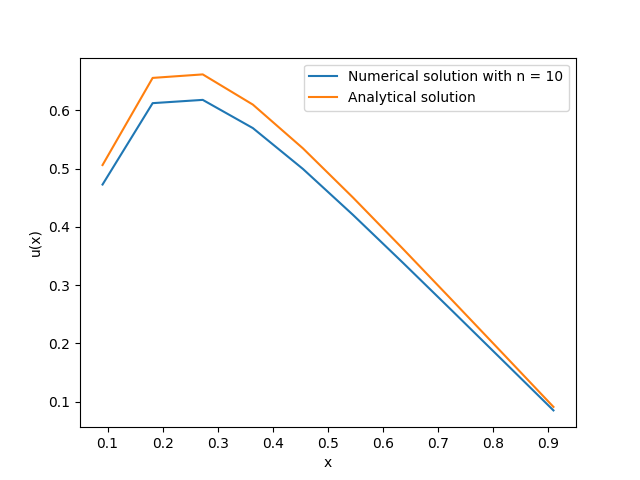
\includegraphics{solution_part_b_n_10_general.png}
	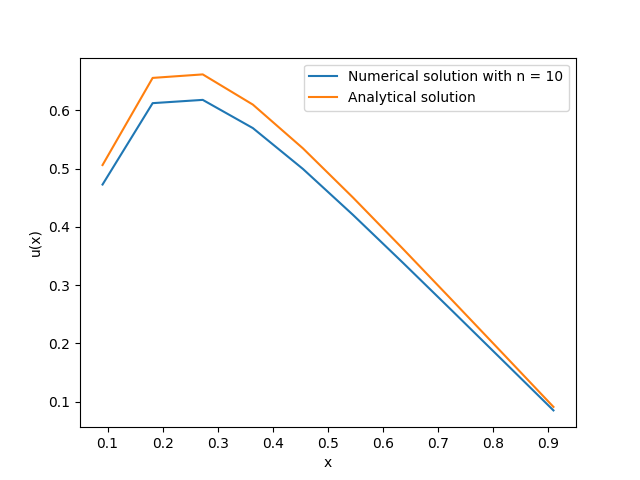
\includegraphics{solution_part_b_n_10_general.png}
	\caption{The figure shows the numerical solution $v(x)$ and the closed-form solution $u(x)$ over the interval $x\in(0,1)$.}
\end{figure}



\end{document} 